
As was discussed in \sec\ref{sec:theory_www_production}, there are other decay
channels of the $WWW$ process besides the fully-leptonic decay channel,
which was the focus of Chapter \ref{sec:www}.  
In fact, one other decay channel for this process has been studied within 
ATLAS. This is the semi-leptonic channel where \wwwlljj. The details of this 
analysis are beyond the scope of this thesis. We can use the results of this channel,
however, along with those for the fully-leptonic decay channel, to obtain a stronger measurement
on the overall SM $WWW$ total cross-section measurement and better 
limits on the aQGC signal than
those reported for just the fully-leptonic 
channel in \sec\ref{sec:measurement} and \sec\ref{sec:aqgc_limit}. 


In this chapter we will first summarize the results of the semi-leptonic study. 
This will be followed by a statistical combination of the fully-leptonic and semi-leptonic
results leading to an improved  
measurement on the SM $WWW$ total cross-section and limits on the 
aQGC signal.
The results of this combination are to be published soon \cite{wwwcomb}.




\section{Search for \wwwlljj}
\label{sec:semilep}


The semi-leptonic analysis uses a selection that is designed
to select events from the decay channel \wwwlljj. As such, 
it requests exactly two leptons and two jets.  The selection is similar
to the one used the same-sign $WW$ vector boson fusion (VBF) production process of
\cite{PhysRevLett.113.141803} with the main difference being that
it requires $|\Delta y(jj)| < 1.5$ and $65 \GeV < m_{jj} < 105 \GeV$
to separate the $WWW$ signal from the same-sign $WW$ VBF signal as can be
seen in \fig\ref{fig:signal_semilep}. The selection used is listed in \tab\ref{tab:selection_2l2j}.
It splits the selection into three separate signal regions based on the final
state lepton flavors: $ee$, $e\mu$, and $e\mu$. The final state leptons
are required to have the same sign.

%\begin{table}[ht]
%\tiny
%\begin{tabular}{c|cccccc} 
\hline 
\hline 
        & \multicolumn{1}{c|}{Signal} & \multicolumn{1}{c|}{$Z$ mass CR} & \multicolumn{1}{c|}{$W$ mass CR} & \multicolumn{1}{c|}{3 Lepton CR} &  \multicolumn{1}{c|}{B-Tagged CR} & \multicolumn{1}{c}{$<2$ jets CR} \\ \hline 
Lepton & \multicolumn{6}{c}{Two same-sign leptons with $p_T>30$ GeV} \\  \hline
3$^{rd}$ lepton veto & \multicolumn{3}{c|}{Yes} & \multicolumn{1}{c|}{No} & \multicolumn{2}{c}{Yes} \\  \hline
Jet & \multicolumn{5}{c|}{$\ge 2$ jets with $p_T>20 (30)$ GeV} & $<2$ jets with $p_T>20 (30)$ GeV \\  
      & \multicolumn{5}{c|}{ and $|\eta|<2.5$} &  and $|\eta|<2.5$ \\  \hline
$m_{\ell \ell'}$  & \multicolumn{6}{c}{$m_{\ell\ell'}>40$ GeV} \\  \hline
$m_{ee}$    & \multicolumn{1}{c|}{$m_{ee}<80$ GeV or}   & \multicolumn{1}{c|}{\multirow{2}{*}{$80<m_{ee}<110$ GeV}} & \multicolumn{4}{c}{$m_{ee}<80$ GeV or} \\  
                   & \multicolumn{1}{c|}{$m_{ee}>110$ GeV}      & \multicolumn{1}{c|}{} & \multicolumn{4}{c}{$m_{ee}>110$ GeV} \\  \hline
$\Delta \eta_{jj}$     & \multicolumn{5}{c|}{$\Delta \eta_{jj}<1.5$} & No \\ \hline 
$m_{jj}$          & \multicolumn{2}{c|}{\multirow{2}{*}{$65<m_{jj}<105$ GeV}} &  \multicolumn{1}{c|}{$m_{jj}<65$ GeV or} &  \multicolumn{2}{c|}{\multirow{2}{*}{$65<m_{jj}<105$ GeV}} &  \multicolumn{1}{c}{\multirow{2}{*}{No}}  \\ 
                       & \multicolumn{2}{c|}{} &  \multicolumn{1}{c|}{$m_{jj}>105$ GeV} &  \multicolumn{2}{c|}{} & \multicolumn{1}{c}{} \\ \hline
$E_T^{miss}$ & \multicolumn{6}{c}{For the $ee$ and $e\mu$ channel, $E_T^{miss}>55$ GeV} \\   \hline
$b$-jet veto & \multicolumn{4}{c|}{Yes} & \multicolumn{1}{c|}{No} & Yes \\  \hline
\hline 
\end{tabular}


%\caption{\label{tab:selection_2l2j} Selection criteria for the signal region and five control regions.}
%\end{table}


\begin{table}[ht]
\begin{center}
\begin{tabular}{|l||c||c||c|}   \hline 
 & \multicolumn{1}{c||}{$e^\pm e^\pm$} & \multicolumn{1}{c||}{$e^\pm \mu^\pm$}    & \multicolumn{1}{c|}{$\mu^\pm \mu^\pm$}  \\ \hline\hline
Lepton & \multicolumn{3}{c|}{Exactly two same-electric-charge leptons with $p_T>30$ GeV} \\ \hline
Jet        & \multicolumn{3}{c|}{At least two jets with $p_T>(20) 30$ GeV and $|\eta|<2.5$} \\ \hline
$m_{\ell\ell}$        & \multicolumn{3}{c|}{$>40$ GeV}  \\ \hline
\MET                      & \multicolumn{2}{c||}{~~~~~~~~~~~~~~~~~~~~~$>55$ GeV~~~~~~~~~~~~~~~~~~~~~~~~} & \multicolumn{1}{c|}{-}  \\  \hline
$m_{jj}$        & \multicolumn{3}{c|}{$65<m_{jj}<105$ GeV}  \\ \hline
$\Delta \eta_{jj}$        & \multicolumn{3}{c|}{$|\Delta \eta_{jj}|<1.5$}  \\ \hline
\multirow{2}{*}{$Z$ veto}        & \multicolumn{1}{c||}{$m_{ee}<80$ GeV or}  & \multicolumn{2}{c|}{\multirow{2}{*}{-}}  \\
                                                  & \multicolumn{1}{c||}{$m_{ee}>110$ GeV}  & \multicolumn{2}{c|}{}  \\ \hline
Third lepton veto                      & \multicolumn{3}{c|}{No third lepton with $p_T>6$ GeV and $|\eta|<2.5$} \\ \hline
$b-$jet veto                              & \multicolumn{3}{c|}{No identified $b-$jets with $p_T>25$ GeV and $|\eta|<4.5$} \\
\hline
\end{tabular}
\end{center}
\caption{Selection criteria for the semi-leptonic channel.}
\label{tab:selection_2l2j}
\end{table}

\begin{table}[ht!]
\centering
\begin{footnotesize}

\begin{tabular}{|c||c|}
	\hline
      Cut Name & Details \\
      \hline
      \hline
      Tau Veto & Remove any events associated with Tau's \\
      \hline
      Lepton Selection & At least 2 leptons with $P_T> 15$ GeV  \\
      \hline
      Jet Selection & At least 2 jets with $P_T> 15$ GeV \\
      \hline
      Same-sign Leptons & Leptons must have the same electric charge \\
      \hline
      Final Lepton Selection & Exactly Two leptons with $P_T > 30$ GeV, $|\eta|<2.5$ \\
      \hline
      $\Delta R_{\ell \ell}$ & $\Delta R_{\ell \ell} > 0.1$ to remove any possible faulty lepton containers \\
      \hline
      $M_{\ell \ell}$ & $M_{\ell \ell} > 40$ GeV \\
      \hline
      Z Veto & $ | M_{ee} - M_Z | < 20$ GeV (only for the $ee$ channel) \\
      \hline
      Final Jet Selection & Leading(Sub) jet $P_T> 30~(20)$ GeV and $|\eta| < 2.5$ \\
      \hline
      $\Delta R_{\ell j}$ & min $\Delta R_{\ell j} > 0.3$ \\
      \hline
      MET & MET $ > 55$ GeV (Not applied for the $\mu\mu$ channel) \\
      \hline
      $b$-jet Veto & Remove any events that contain any $b$-tagged jets \\
      \hline
      $\Delta R_{jj}$ & $\Delta R_{j j} < 1.5$ to make sure that the two jets come from the $W$ boson decay \\ 
      \hline
      $W$ mass window cut & Two leading jets should have 65 GeV $<M_{jj}<105$ GeV  \\
      \hline
      jet-jet rapidity & $|\Delta y(jj)| < 1.5$ \\
      \hline

\end{tabular}


\end{footnotesize}
\caption{Description of fiducial selection for each of the semi-leptonic channels.  }
\label{tab:fiducial_selection_2l2j}
\end{table}

The signal is generated using \madgraph~with the same setup as in \sec\ref{sec:signal}.
Thus, the total cross-section is the same as in \eqn\eqref{eq:total_www_xsec}.
The fiducial cross-sections are determined in a similar fashion to that in 
\sec\ref{sec:fiducial} but using the fiducial selection listed in \tab\ref{tab:fiducial_selection_2l2j}.
The fiducial cross-section is 
\begin{equation}
\sigma^{\textrm{Fiducial,Semi-lep}}_{\textrm{Theory}}= 306\pm6.73 ~(\textrm{Stat.}) ~^{+15.3}_{-8.57} ~(\textrm{PDF}) ~\pm 3.05 ~(\textrm{Scale}) ~\textrm{ab} %uncertainty?
\end{equation}

\begin{figure}[h]
  \begin{center}
    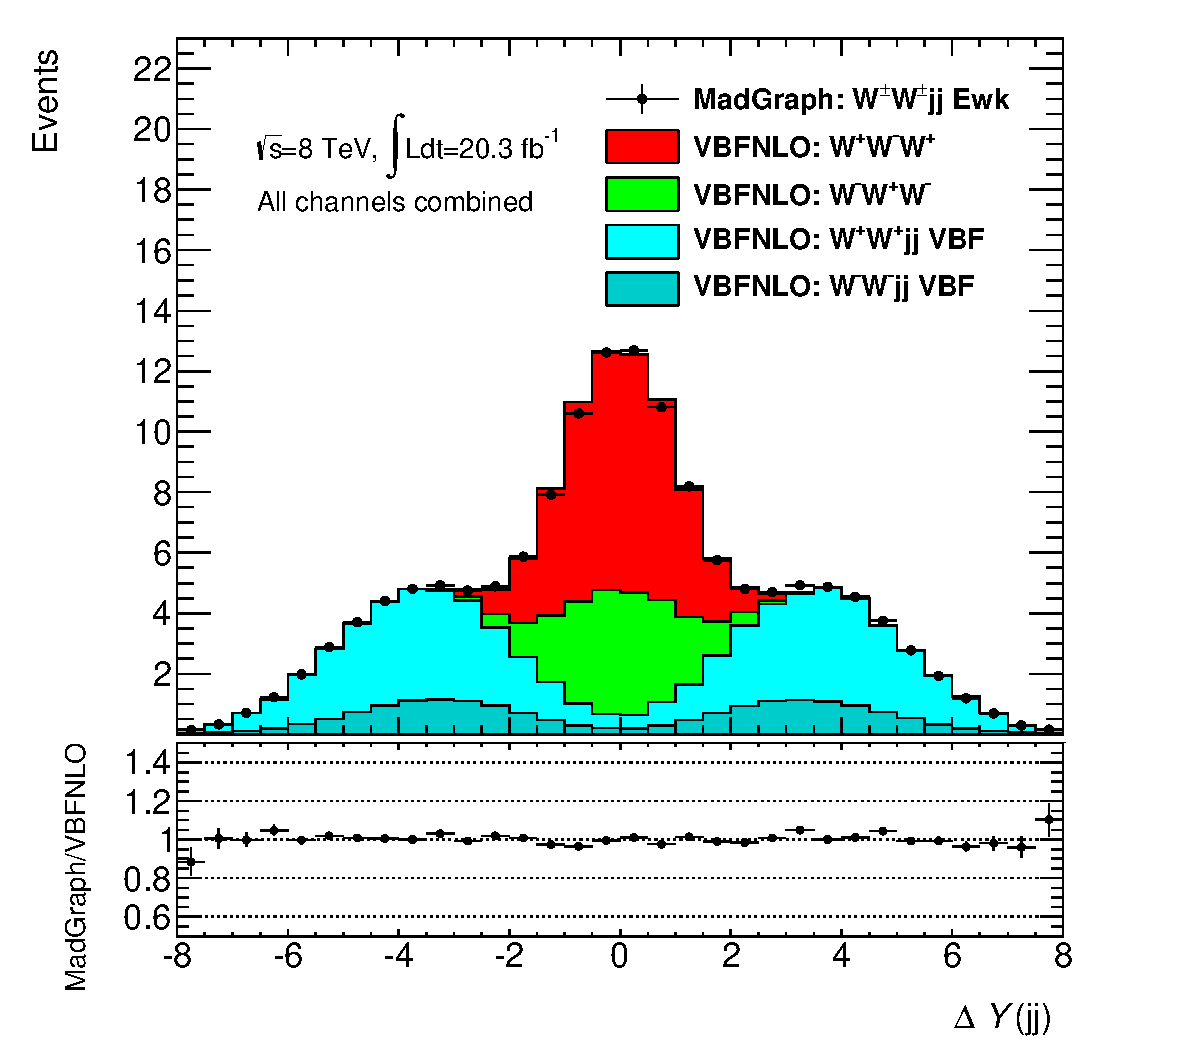
\includegraphics[width=0.45\textwidth]{figures/combination/dY2j_linear_ratio.pdf}
    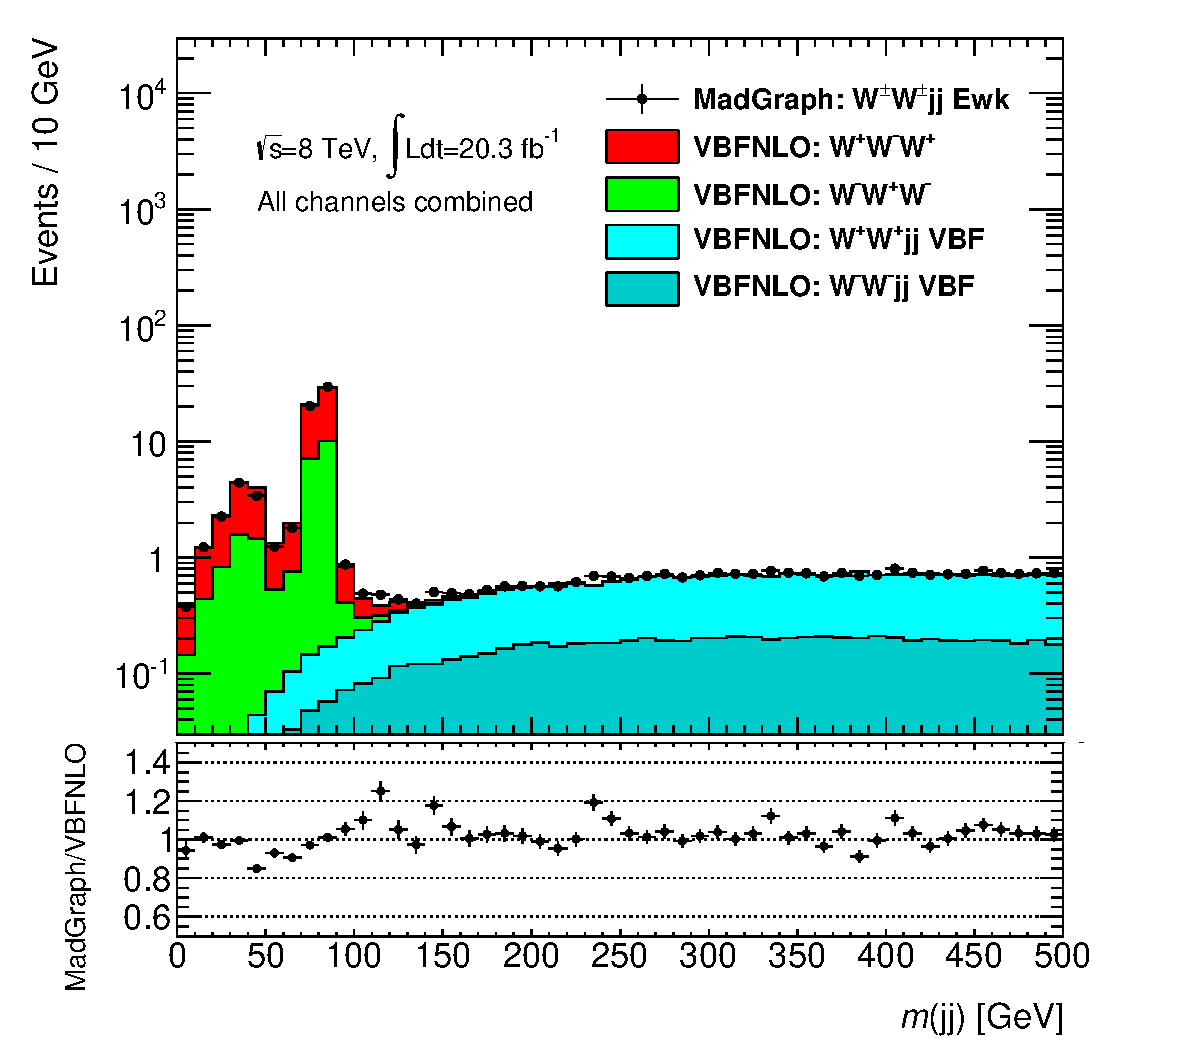
\includegraphics[width=0.45\textwidth]{figures/combination/TwojM_log_ratio.pdf}
  \end{center}
  \caption{Comparison of $\Delta Y(jj)$ and $M_{jj}$ distributions between VBFNLO and MadGraph LO events with two same-sign leptons and two jets in the final state. }
  \label{fig:signal_semilep} 
\end{figure}


The backround is estimated in a similar way to \sec\ref{sec:bg_estimates}. The $WZ$, 
$V\gamma$, and other same-sign ($Z$,$WW$,$ZZ$, $\ttV$, etc) backgrounds are predicted
using MC. The charge mis-identification background is evaluated using a data-driven method
where the rates are derived in a similar way as in \sec\ref{sec:chargemisd_rates}
but are instead applied as weights on the data.
The fake lepton background is also evaluated using the data but uses a form factor method
instead of the generalized matrix method of \sec\ref{sec:mxm}.


\begin{table}[ht!]
\centering
\renewcommand{\tabcolsep}{2pt}
\begin{tabular}{c|rclrclrcl}
\hline 
\hline 
 & \multicolumn{3}{c}{$e^\pm e^\pm$} & \multicolumn{3}{c}{$e^\pm \mu^\pm$} & \multicolumn{3}{c}{$\mu^\pm \mu^\pm$}\\ 
 \hline
Fake & 0.96 &$\pm$& 0.15 $^{+0.39}_{-0.39}$  & 2.04 &$\pm$& 0.22 $^{+0.89}_{-0.89}$  & 0.43 &$\pm$& 0.06 $^{+0.25}_{-0.25}$ \\[0.2cm] 
$WZ$ & 0.74 &$\pm$& 0.13 $^{+0.44}_{-0.44}$  & 2.77 &$\pm$& 0.27 $^{+0.66}_{-0.65}$  & 3.28 &$\pm$& 0.29 $^{+0.66}_{-0.71}$ \\[0.2cm] 
$V\gamma$ & 0.75 &$\pm$& 0.35 $^{+0.21}_{-0.18}$  & 2.48 &$\pm$& 0.68 $^{+0.73}_{-0.74}$  & 0.0 &$\pm$& 0.0 $^{+0.0}_{-0.0}$ \\[0.2cm] 
Charge Mis-identification & 1.13 &$\pm$& 0.13 $^{+0.24}_{-0.24}$  & 0.74 &$\pm$& 0.08 $^{+0.16}_{-0.16}$  & 0.0 &$\pm$& 0.0 $^{+0.0}_{-0.0}$ \\[0.2cm] 
Other Same-Sign & 0.46 &$\pm$& 0.05 $^{+0.16}_{-0.15}$  & 1.33 &$\pm$& 0.1 $^{+0.37}_{-0.38}$  & 1.33 &$\pm$& 0.15 $^{+0.38}_{-0.32}$ \\[0.2cm] 
Signal & 0.46 &$\pm$& 0.03 $^{+0.07}_{-0.07}$  & 1.35 &$\pm$& 0.05 $^{+0.19}_{-0.19}$  & 1.65 &$\pm$& 0.06 $^{+0.3}_{-0.3}$ \\[0.2cm] 
\hline 
Total background  & 4.04 &$\pm$& 0.42 $^{+0.69}_{-0.68}$  & 9.36 &$\pm$& 0.77 $^{+1.39}_{-1.39}$  & 5.04 &$\pm$& 0.34 $^{+0.8}_{-0.82}$ \\[0.2cm] 
Total predicted & 4.51 &$\pm$& 0.43 $^{+0.69}_{-0.69}$  & 10.72 &$\pm$& 0.77 $^{+1.4}_{-1.4}$  & 6.69 &$\pm$& 0.34 $^{+0.85}_{-0.87}$ \\ \hline 
Data & \multicolumn{3}{c}{0} & \multicolumn{3}{c}{15} & \multicolumn{3}{c}{6}\\ 
\hline 
\end{tabular}


\caption{A summary of the expected yields compared to data for all 
three signal regions in the semi-leptonic analysis channel.  
Statistical uncertainties are shown 
as a symmetric uncertainty on the central value. Systematic uncertainties 
are shown as an asymmetric uncertainty and are shown
after taking the quadrature sum of all individual uncertainties. 
In the actual analysis, each systematic uncertainty is
treated as an individual nuisance parameter and are NOT added in quadrature.  
The presentation here serves only as a demonstration
of the overall size of the systematic uncertainties for each source in the 
individual signal regions.}
\label{tab:yields_2l2j}
\end{table}

\begin{table}[ht!]
\centering

\renewcommand{\arraystretch}{1.5}
\begin{tabular}{c||ccc|ccc}
\hline
\multirow{2}{*}{Source of Uncertainty} & \multicolumn{3}{c|}{Signal} & \multicolumn{3}{c}{Backgound} \\
        &$e^\pm e^\pm$ &$e^\pm \mu^\pm$ &$\mu^\pm \mu^\pm$ &$e^\pm e^\pm$ &$e^\pm \mu^\pm$ &$\mu^\pm \mu^\pm$ \\ \hline  \hline
Electron  &$^{+3.24}_{-3.47}$  &$^{+0.98}_{-1.17}$  &$^{+0.0}_{-0.07}$  &$^{+0.9}_{-0.93}$  &$^{+1.72}_{-0.94}$  &$^{+0.09}_{-0.0}$\\
Muon  &$^{+0.0}_{-0.0}$  &$^{+1.25}_{-1.18}$  &$^{+1.39}_{-1.42}$  &$^{+0.39}_{-0.39}$  &$^{+1.25}_{-1.22}$  &$^{+5.26}_{-6.17}$\\
MET  &$^{+2.44}_{-4.58}$  &$^{+0.95}_{-1.67}$  &$^{+0.63}_{-0.15}$  &$^{+3.47}_{-2.26}$  &$^{+3.39}_{-3.39}$  &$^{+2.34}_{-1.22}$\\
Flavor Tagging  &$^{+2.15}_{-2.16}$  &$^{+2.16}_{-2.17}$  &$^{+2.25}_{-2.26}$  &$^{+1.27}_{-1.31}$  &$^{+2.2}_{-2.34}$  &$^{+2.68}_{-2.75}$\\
Jet Energy Scale  &$^{+5.23}_{-5.66}$  &$^{+6.58}_{-5.84}$  &$^{+6.2}_{-6.08}$  &$^{+8.18}_{-8.28}$  &$^{+6.42}_{-6.95}$  &$^{+6.13}_{-6.33}$\\
Jet Energy Resolution  &$^{+13.13}_{-13.13}$  &$^{+12.12}_{-12.12}$  &$^{+16.57}_{-16.57}$  &$^{+12.34}_{-12.34}$  &$^{+8.72}_{-8.72}$  &$^{+0.94}_{-0.94}$\\
Luminosity  &$^{+1.9}_{-1.9}$  &$^{+1.9}_{-1.9}$  &$^{+1.9}_{-1.9}$  &$^{+0.92}_{-0.92}$  &$^{+1.34}_{-1.34}$  &$^{+1.74}_{-1.74}$\\
Theory  &$^{+4.0}_{-7.0}$  &$^{+4.0}_{-7.0}$  &$^{+4.0}_{-7.0}$  &$^{+8.69}_{-8.69}$  &$^{+12.44}_{-12.44}$  &$^{+15.78}_{-15.78}$\\
\hline\hline 
\end{tabular}


\caption{Categorized systematic uncertainties 
for signal and background predictions in all three signal regions
of the semi-leptonic analysis channel.
All uncertainties are shown as a percentage of the nominal
prediction.  }
\label{tab:sys_2l2j}
\end{table}

\begin{table}[ht!]
\centering
\begin{tabular}{|c||c|c|c|}
\hline
%& Channel & Signal Efficiency, $\varepsilon_i$  & Acceptance ($\times 10^{-4}$), $A_i$\\
 Channel & $C_i$   & Fiducial Cross-section [ab]\\
%&         & $\varepsilon_i$    &  $A_i$ \\
\hline\hline
$e^\pm e^\pm$ &  $0.450 \pm .036$ & $50.4 \pm 2.5$\\
$e^\pm \mu^\pm$ &  $0.531 \pm .026$ & $125.2 \pm 3.8$\\
$\mu^\pm \mu^\pm$ &  $0.626 \pm .029$ & $129.9  \pm 3.9$ \\
\hline
\end{tabular}


\caption{Correction factors, $C_i$, and fiducial cross-sections derived
separately for each signal region in the semi-leptonic analysis channel. 
Correction factors and  fiducial cross-sections are determined
using \madgraph.}
\label{tab:inputs_2l2j}
\end{table}

The resulting signal and background predictions and overall systematic uncertainties,
as well as the observed data events,
are shown for each semi-leptonic signal region in \tab\ref{tab:yields_2l2j}. Systematics
are determined in the same way as in \sec\ref{sec:systematics} except for the charge
mis-identification backgrounds and fake backgrounds which evaluate different systematics due
to the different estimation methods used. The systematics for the semi-leptonic
channel are summarized in \tab\ref{tab:sys_2l2j}. The fiducial cross-sections
and correction factors (like in \eqn\eqref{eq:cfactor}) are presented in \tab\ref{tab:inputs_2l2j}.

Semi-leptonic aQGC inputs...

More details can be found in \cite{wwwcomb} once published.

\section{Combined Cross-section Measurement}
\label{sec:combined_measurement}

The cross-section measurement using the combination of the semi-leptonic
and fully-leptonic analysis channels is performed to 
measure the total cross-section of the $WWW$ process. 
The same expectation, likelihood, and profile likelihood
ratios are used as in \eqn\eqref{eq:poisson_expectation},
\eqn\eqref{eq:poisson_likelihood}, and
\eqn\eqref{eq:profile_likelihood_ratio}, respectively.
The same methodology for extracting the measured fiducial
cross-section from
\sec\ref{sec:measurement} is used for extracting the combined
cross-section measurement except that the semi-leptonic channel
inputs are included along with the fully-leptonic channel
and that the measurement is extrapolated to the total
cross-section.
For the fully-leptonic channel,
the fiducial cross-section and C-factor inputs 
are taken from \tab\ref{tab:inputs_3l}
while the semi-leptonic channel inputs are taken from 
\tab\ref{tab:inputs_2l2j}.
The combined measurement on the signal strength, $\mu$, is translated
into a measurement on the total cross-section using the relation
\begin{equation}
\sigma^{\textrm{Total}}_{\textrm{Observed}} = \frac{\mu}{A} \sum_{i\in \textrm{Channels}} \sigma^{\textrm{Fiducial}}_i
\label{eq:sigmatot}
\end{equation}
where $A$ is the total acceptance which is the sum of the 
acceptance in each channel, $A_i$:
\begin{equation}
A = \sum_i A_i
\end{equation}
and where $A_i$ is computed as
\begin{equation}
A_i = \frac{ \sigma^{\textrm{Fiducial}}_i }{ \sigma^{\textrm{Total}}}
\end{equation}
The $\sigma^{\textrm{Fiducial}}_i $ are simply the fiducial
cross-sections in each channel, $i$,  taken from
\tab\ref{tab:inputs_3l} and \tab\ref{tab:inputs_2l2j}
and $\sigma^{\textrm{Total}}$ is the expected total cross-section
in \eqn\eqref{eq:total_www_xsec}, reprinted here for convenience:
\begin{equation}
\sigma^{\textrm{Total}}_{\textrm{Theory}}= 241.47\pm0.13 ~(\textrm{Stat.}) ~^{+10.33}_{-6.08} ~(\textrm{PDF}) ~\pm 6.3 ~(\textrm{Scale}) ~\textrm{fb} %uncertainty?
\end{equation}
The acceptance values for both the semi-leptonic and fully-leptonic channels 
are summarized here in \tab\ref{tab:acceptance}.
The total acceptance is found to be $A = 2.547 \times 10^{-3} \pm 0.039 \times 10^{-3}$.


\begin{table}[ht!]
\centering
\begin{tabular}{|cc||c|}
\hline
%& Channel & Signal Efficiency, $\varepsilon_i$  & Acceptance ($\times 10^{-4}$), $A_i$\\
& Channel & $A_i$ ($\times 10^{-3}$)\\
%&         & $\varepsilon_i$    &  $A_i$ \\
\hline\hline
\multirow{3}{*}{Fully-leptonic} & 0 SFOS & $0.512 \pm .019$ \\
				& 1 SFOS & $0.567 \pm .020$ \\
                                & 2 SFOS & $0.202 \pm .012$ \\
\hline
\multirow{3}{*}{Semi-leptonic} & $ee$     & $0.209 \pm .011$\\
                               & $e\mu$   & $0.519 \pm .016$\\
                               & $\mu\mu$ & $0.538 \pm .016$\\
\hline
\end{tabular}

\caption{Acceptance values, $A_i$, derived separately for each signal region. 
The sum of all of the acceptance
in each bin is used to compute the overall acceptance, $A$. 
Only statistical uncertainties are shown.}
\label{tab:acceptance}
\end{table}


The distribution of $q_0$ is shown 
in Fig.~\ref{fig:stat_measurement_significance} for the combination.  
The observed null p-value 
is found to be 0.1657 ($0.971~\sigma$) with an 
expected of 0.152 ($1.026~\sigma$).

%this is with reduced systematics. what is the effect of adding or removing more?
%plot should be redone with a bigger range
\begin{figure}[ht!]
\centering
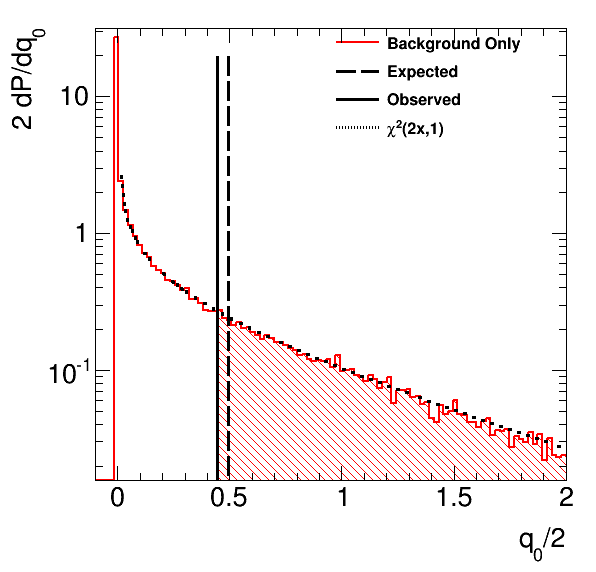
\includegraphics[width=0.70\columnwidth]{figures/combination/significance.png}
\caption{PDF of the background only hypothesis as a function of $q_0$ for the combination of all three channels. PDFs are determined 
using toy MC. The dashed black line represents the expected value of $q_0$ while the solid black line represents the observed value of $q_0$ seen in the data. The shaded area to the right
of this line represents the null p-value or the 
integral of the background hypothesis in the signal-like region.
The dotted black curve shows a $\chi^2$ distribution for 1 degree of freedom with which 
it can be seen is a good approximation of the 
the background only PDF.}
\label{fig:stat_measurement_significance}
\end{figure}

The negative log likelihood contour is shown
for the combination of all six channels in 
Fig.~\ref{fig:stat_measurement_interval_combination}.
The expected value and uncertainties for the total cross-section is:
\begin{equation}
\sigma^{\textrm{Total}}_{\textrm{Expected}} = 241.47 ~ ^{+232}_{-199} \stat ~^{+152}_{-153}\syst ~\textrm{fb}
\end{equation}
while the observed total cross-section is:
\begin{equation}
\sigma^{\textrm{Total}}_{\textrm{Observed}} = 227.03 ~ ^{+202}_{-198} \stat ~^{+154}_{-160} \syst ~\textrm{fb}
\end{equation}

%Pulls and correlations

\begin{figure}[ht!]
\centering
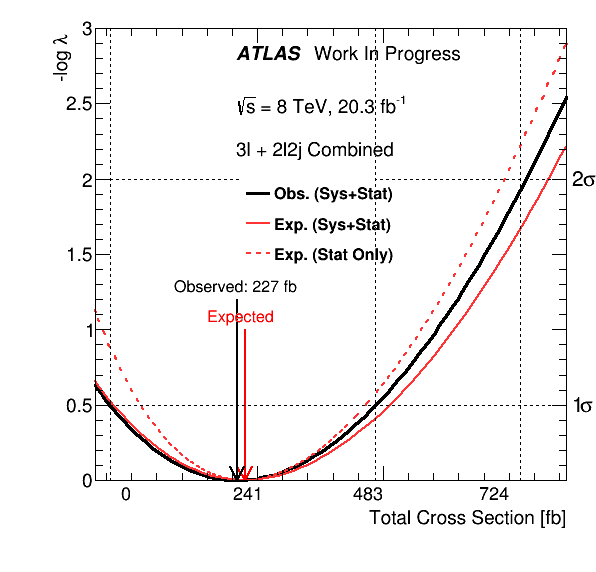
\includegraphics[scale=0.7]{figures/combination/interval_comb.png}
\caption{The profile likelihood contours evaluated as a function of the signal strength
for the combination of all three channels. 
The observed (black) and expected (red) contours are shown when considering only statistical uncertainty (dashed line) and when considering both statistical and systematic uncertainties (solid line).
The dotted black
lines pinpoint the location of the $1~\sigma$ and $2~\sigma$ total Gaussian uncertainties
on the measurement of the signal strength which corresponds to the minimum value of the contour.}
\label{fig:stat_measurement_interval_combination}
\end{figure}







%Acceptnace
%combined tables
%Measurement using same framework

\section{Combined aQGC Limits}
\label{sec:combined_aqgc}


\begin{table}[h!]
  \begin{center}
   \begin{tabular}{  |l| c | c c c | c c c | }
      \hline
      %&$\Lambda$& \multicolumn{6}{c|}{Expected Limit}  \\
      &$\Lambda$& \multicolumn{3}{c|}{Limits on F$_{s0}$ [$10^3~\TeV^{-4}$]}& \multicolumn{3}{c|}{Limits on F$_{s1}$ [$10^3~\TeV^{-4}$]}  \\
      &[\GeV]&  Lower & Upper & Measured & Lower & Upper & Measured  \\
      \hline
\multirow{5}{*}{Expected}      &500  & -8.12 & 8.92 & --- & -10.04 & 12.91 & --- \\ 
      &1000 & -3.7 & 4.16 & --- & -5.21 & 6.19 & --- \\ 
      &2000 & -2.35 & 2.57 & --- &-3.33 & 4.02 & --- \\ 
      &3000 & -1.87 & 2.24 & --- &-2.94 & 3.58 & --- \\ 
      &$\infty$ & -1.59 & 1.91 & --- & -2.54 & 3.09  & --- \\ 
      \hline \hline
\multirow{5}{*}{Observed}      &500  & -7.66 & 8.45 & 0.35  & -10.08 & 12.22 & 1.11 \\
      &1000 &  -3.11 & 3.87 & 0.40 & -4.77 & 5.81 & 0.85  \\
      &2000 &  -1.92 & 2.40 & 0.322  & -2.90 & 3.69 & 0.49 \\
      &3000 &  -1.6 & 2.09 & 0.37 & -2.48 & 3.18 & 0.47  \\
      &$\infty$& -1.27 & 1.76 & 0.34 & -2.10 & 2.71  & 0.40\\ 
      \hline
\end{tabular}


    \caption{Expected and observed one-dimensional limits on the aQGC Parameters.}
    \label{tab:aqgc_combined_1d}

  \end{center}
\end{table}


Combined limits on the aQGC signal use the same methodology
as in \sec\ref{sec:aqgc_limit} except that the inputs from the semi-leptonic
channel, described in \sec\ref{sec:semilep}, are included as well.
The resulting one-dimensional limits are listed in \tab\ref{tab:aqgc_combined_1d}
while the two-dimensional limts are shown in \fig\ref{fig:aqgc_combined_2d}.


\begin{figure}[h!]
\begin{center}

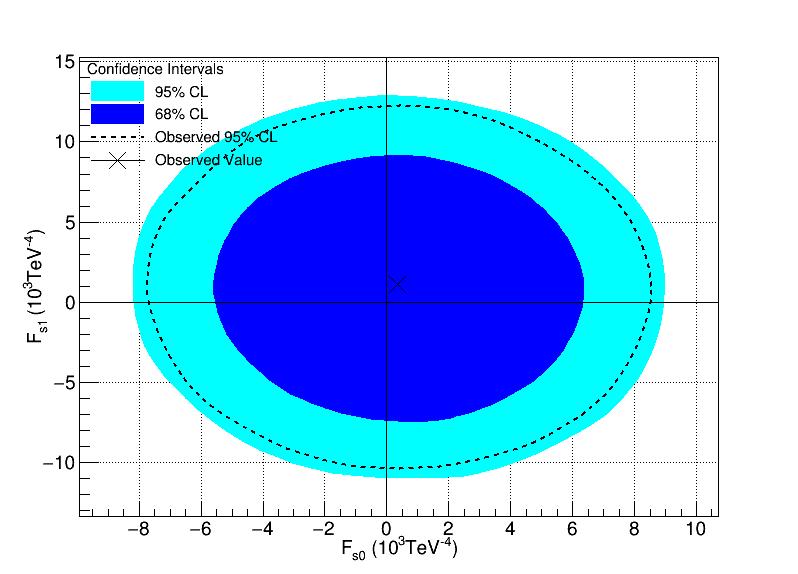
\includegraphics[width=0.45\textwidth]{figures/combination/Comb500-Lim.png}
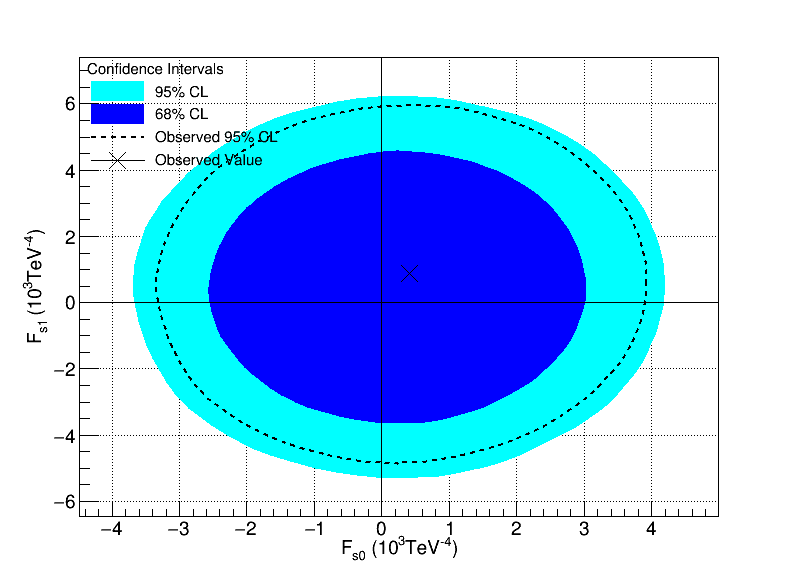
\includegraphics[width=0.45\textwidth]{figures/combination/Comb100-Lim.png}\\
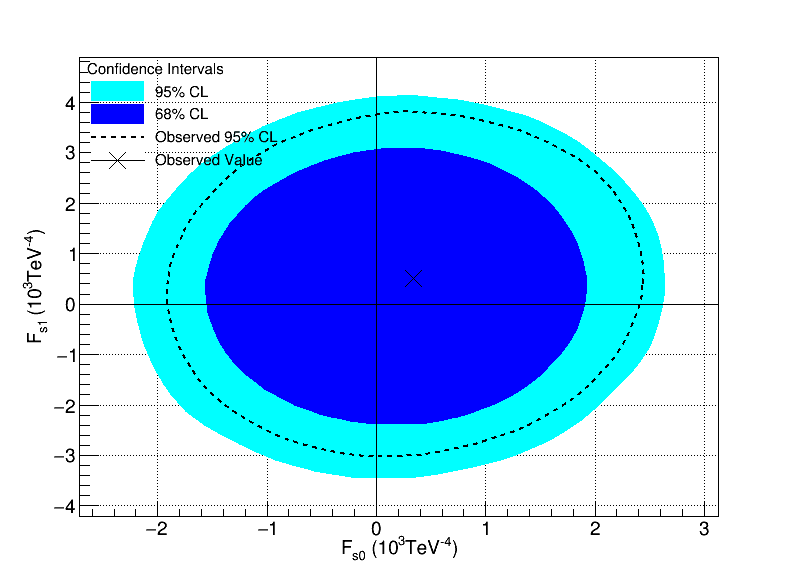
\includegraphics[width=0.45\textwidth]{figures/combination/Comb200-Lim.png}
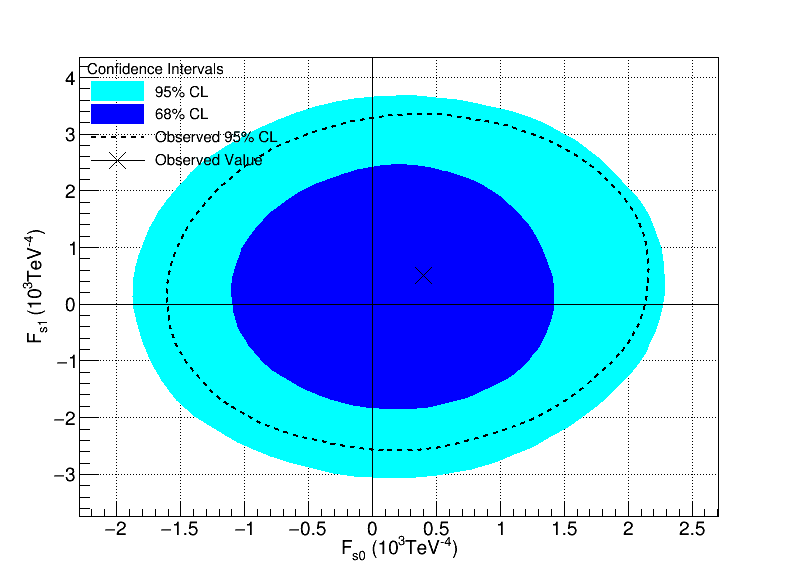
\includegraphics[width=0.45\textwidth]{figures/combination/Comb300-Lim.png}\\
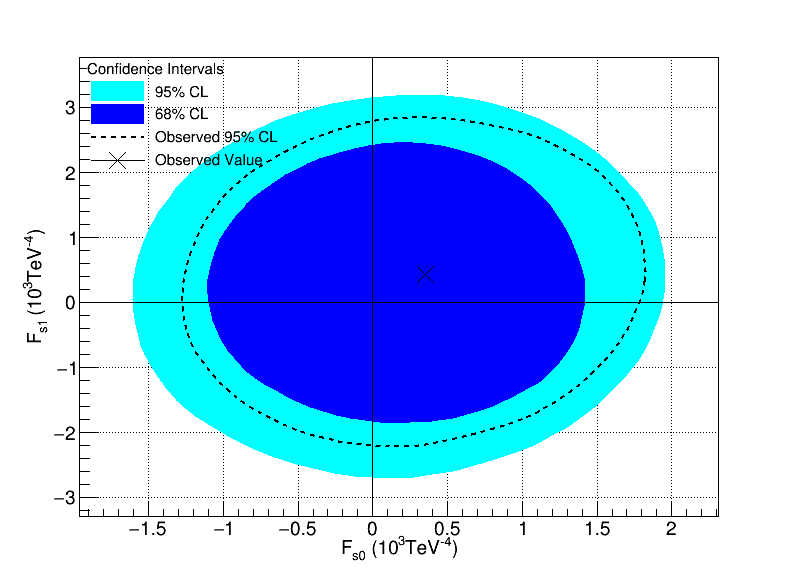
\includegraphics[width=0.45\textwidth]{figures/combination/CombUnit-Lim.png}
\end{center}
\caption{Two-dimensional limits at 95\% CL on the combination for the non-unitarized case (Top Left)
and three different choices of the unitarization scale, $\Lambda$:
3~\TeV~(Top Right), 2~\TeV~(Middle Left), 1~\TeV~(Middle Right), and 0.5~\TeV~(Bottom Center).}

 \label{fig:aqgc_combined_2d}
 \end{figure}



